

\tikzset{every picture/.style={line width=0.75pt}} %set default line width to 0.75pt        

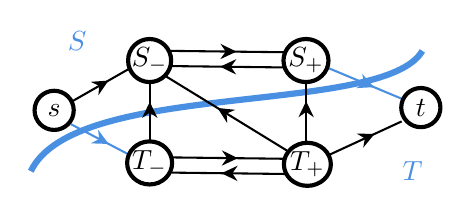
\begin{tikzpicture}[x=0.5pt,y=0.5pt,yscale=-1,xscale=1]
%uncomment if require: \path (0,219); %set diagram left start at 0, and has height of 219

%Curve Lines [id:da293114086641606] 
\draw [color={rgb, 255:red, 74; green, 144; blue, 226 }  ,draw opacity=1 ][line width=2.25]    (44.5,171) .. controls (76.5,104) and (299.5,132) .. (327.5,84) ;
%Straight Lines [id:da07818022990875795] 
\draw [color={rgb, 255:red, 0; green, 0; blue, 0 }  ,draw opacity=1 ][line width=0.75]    (115.5,97) -- (73.5,121) ;
\draw [shift={(100.66,105.48)}, rotate = 150.26] [fill={rgb, 255:red, 0; green, 0; blue, 0 }  ,fill opacity=1 ][line width=0.08]  [draw opacity=0] (11.61,-5.58) -- (0,0) -- (11.61,5.58) -- (7.71,0) -- cycle    ;
%Straight Lines [id:da13447323458917793] 
\draw [color={rgb, 255:red, 74; green, 144; blue, 226 }  ,draw opacity=1 ][line width=0.75]    (115.5,159) -- (73.5,137) ;
\draw [shift={(100.79,151.29)}, rotate = 207.65] [fill={rgb, 255:red, 74; green, 144; blue, 226 }  ,fill opacity=1 ][line width=0.08]  [draw opacity=0] (11.61,-5.58) -- (0,0) -- (11.61,5.58) -- (7.71,0) -- cycle    ;
%Straight Lines [id:da8494415517252689] 
\draw [color={rgb, 255:red, 74; green, 144; blue, 226 }  ,draw opacity=1 ][line width=0.75]    (313.5,119) -- (258.5,96) ;
\draw [shift={(292.55,110.24)}, rotate = 202.69] [fill={rgb, 255:red, 74; green, 144; blue, 226 }  ,fill opacity=1 ][line width=0.08]  [draw opacity=0] (11.61,-5.58) -- (0,0) -- (11.61,5.58) -- (7.71,0) -- cycle    ;
%Straight Lines [id:da07398074829543488] 
\draw [color={rgb, 255:red, 0; green, 0; blue, 0 }  ,draw opacity=1 ][line width=0.75]    (312.5,135) -- (260.5,159) ;
\draw [shift={(292.95,144.02)}, rotate = 155.22] [fill={rgb, 255:red, 0; green, 0; blue, 0 }  ,fill opacity=1 ][line width=0.08]  [draw opacity=0] (11.61,-5.58) -- (0,0) -- (11.61,5.58) -- (7.71,0) -- cycle    ;
%Straight Lines [id:da19965646081311195] 
\draw [color={rgb, 255:red, 0; green, 0; blue, 0 }  ,draw opacity=1 ][line width=0.75]    (227.5,85) -- (144.5,84) ;
\draw [shift={(193.1,84.59)}, rotate = 180.69] [fill={rgb, 255:red, 0; green, 0; blue, 0 }  ,fill opacity=1 ][line width=0.08]  [draw opacity=0] (11.61,-5.58) -- (0,0) -- (11.61,5.58) -- (7.71,0) -- cycle    ;
%Straight Lines [id:da5020627943874022] 
\draw [color={rgb, 255:red, 0; green, 0; blue, 0 }  ,draw opacity=1 ][line width=0.75]    (228.5,96) -- (145.5,95) ;
\draw [shift={(181.4,95.43)}, rotate = 0.69] [fill={rgb, 255:red, 0; green, 0; blue, 0 }  ,fill opacity=1 ][line width=0.08]  [draw opacity=0] (11.61,-5.58) -- (0,0) -- (11.61,5.58) -- (7.71,0) -- cycle    ;
%Straight Lines [id:da3615258313224192] 
\draw [color={rgb, 255:red, 0; green, 0; blue, 0 }  ,draw opacity=1 ][line width=0.75]    (228.5,162) -- (145.5,161) ;
\draw [shift={(194.1,161.59)}, rotate = 180.69] [fill={rgb, 255:red, 0; green, 0; blue, 0 }  ,fill opacity=1 ][line width=0.08]  [draw opacity=0] (11.61,-5.58) -- (0,0) -- (11.61,5.58) -- (7.71,0) -- cycle    ;
%Straight Lines [id:da9852604392093721] 
\draw [color={rgb, 255:red, 0; green, 0; blue, 0 }  ,draw opacity=1 ][line width=0.75]    (229.5,173) -- (146.5,172) ;
\draw [shift={(182.4,172.43)}, rotate = 0.69] [fill={rgb, 255:red, 0; green, 0; blue, 0 }  ,fill opacity=1 ][line width=0.08]  [draw opacity=0] (11.61,-5.58) -- (0,0) -- (11.61,5.58) -- (7.71,0) -- cycle    ;
%Straight Lines [id:da8921257697911721] 
\draw [color={rgb, 255:red, 0; green, 0; blue, 0 }  ,draw opacity=1 ][line width=0.75]    (130.5,107) -- (130.5,149) ;
\draw [shift={(130.5,120.9)}, rotate = 90] [fill={rgb, 255:red, 0; green, 0; blue, 0 }  ,fill opacity=1 ][line width=0.08]  [draw opacity=0] (11.61,-5.58) -- (0,0) -- (11.61,5.58) -- (7.71,0) -- cycle    ;
%Straight Lines [id:da2647924953727303] 
\draw [color={rgb, 255:red, 0; green, 0; blue, 0 }  ,draw opacity=1 ][line width=0.75]    (243.5,106) -- (243.5,149) ;
\draw [shift={(243.5,120.4)}, rotate = 90] [fill={rgb, 255:red, 0; green, 0; blue, 0 }  ,fill opacity=1 ][line width=0.08]  [draw opacity=0] (11.61,-5.58) -- (0,0) -- (11.61,5.58) -- (7.71,0) -- cycle    ;
%Straight Lines [id:da598001554052235] 
\draw [color={rgb, 255:red, 0; green, 0; blue, 0 }  ,draw opacity=1 ][line width=0.75]    (141.5,102) -- (229.5,156) ;
\draw [shift={(179.45,125.29)}, rotate = 31.53] [fill={rgb, 255:red, 0; green, 0; blue, 0 }  ,fill opacity=1 ][line width=0.08]  [draw opacity=0] (11.61,-5.58) -- (0,0) -- (11.61,5.58) -- (7.71,0) -- cycle    ;

% Text Node
\draw  [line width=1.5]   (130.38, 91) circle [x radius= 15.56, y radius= 15.56]   ;
\draw (130.38,91) node   [align=left] {$\displaystyle S_{-}$};
% Text Node
\draw  [line width=1.5]   (130.38, 165) circle [x radius= 16.26, y radius= 15.56]   ;
\draw (130.38,165) node   [align=left] {$\displaystyle T_{-}$};
% Text Node
\draw  [line width=1.5]   (243.38, 91) circle [x radius= 16.26, y radius= 15.56]   ;
\draw (243.38,91) node   [align=left] {$\displaystyle S_{+}$};
% Text Node
\draw  [line width=1.5]   (244.38, 166) circle [x radius= 16.97, y radius= 15.56]   ;
\draw (244.38,166) node   [align=left] {$\displaystyle T_{+}$};
% Text Node
\draw  [line width=1.5]   (61.38, 127) circle [x radius= 14.15, y radius= 14.15]   ;
\draw (61.38,127) node   [align=left] {$\displaystyle s$};
% Text Node
\draw  [line width=1.5]   (326.38, 125) circle [x radius= 14.15, y radius= 14.15]   ;
\draw (326.38,125) node   [align=left] {$\displaystyle t$};
% Text Node
\draw (69,68) node [anchor=north west][inner sep=0.75pt]  [color={rgb, 255:red, 74; green, 144; blue, 226 }  ,opacity=1 ] [align=left] {$\displaystyle S$};
% Text Node
\draw (311,162) node [anchor=north west][inner sep=0.75pt]  [color={rgb, 255:red, 74; green, 144; blue, 226 }  ,opacity=1 ] [align=left] {$\displaystyle T$};


\end{tikzpicture}

